\documentclass[usenatbib,usegraphicx,letterpaper]{mn2e}
\usepackage[totalwidth=480pt,totalheight=680pt]{geometry}

\usepackage{amssymb}
\usepackage{epsfig}
\usepackage{amsmath}
\usepackage{color}

\bibliographystyle{mn2e}

%-------- journals
\newcommand{\araa}{ARAA~}
\newcommand{\apj}{ApJ~}
\newcommand{\apjl}{ApJL~}
\newcommand{\apjs}{ApJS~}
\newcommand{\mnras}{MNRAS~}
\newcommand{\nat}{Nature~}
\newcommand{\physrep}{Phys. Rep.~}
\newcommand{\aj}{AJ~}
\newcommand{\pasp}{ASP~}

%%%% Misc %%%
\newcommand{\beq}{\begin{equation}}
\newcommand{\eeq}{\end{equation}}
\newcommand{\beqray}{\begin{eqnarray}}
\newcommand{\eeqray}{\end{eqnarray}}

\newcommand{\ben}{\begin{enumerate}}
\newcommand{\een}{\end{enumerate}}
\newcommand{\bit}{\begin{itemize}}
\newcommand{\eit}{\end{itemize}}

%%%%%%%%  galaxy properties  %%%%%%%%
\newcommand{\rhalf}{R_{1/2}}
\newcommand{\rhalfdisk}{R_{1/2}^{\rm disk}}
\newcommand{\rhalfbulge}{R_{1/2}^{\rm bulge}}
\newcommand{\adisk}{A_{\rm disk}}
\newcommand{\abulge}{A_{\rm bulge}}
\newcommand{\alphadisk}{\alpha_{\rm disk}}
\newcommand{\alphabulge}{\alpha_{\rm bulge}}
\newcommand{\sigmarhalf}{\sigma_{\rm R_{1/2}}}
\newcommand{\bt}{{\rm B/T}}
\newcommand{\mstar}{M_{\ast}}
\newcommand{\ssfr}{{\rm sSFR}}
\newcommand{\sfr}{{\rm SFR}}

%%%%%%%%  halo properties  %%%%%%%%
\newcommand{\halospin}{\lambda_{\rm halo}}
\newcommand{\mvir}{M_{\rm vir}}
\newcommand{\macc}{M_{\rm acc}}
\newcommand{\mpeak}{M_{\rm peak}}
\newcommand{\zpeak}{z_{M_{\rm peak}}}
\newcommand{\mhalo}{M_{\rm halo}}
\newcommand{\rvir}{R_{\rm vir}}
\newcommand{\rmpeak}{R_{\rm M_{peak}}}
\newcommand{\vmaxmpeak}{V_{\rm peak}}
\newcommand{\vmax}{V_{\rm max}}
\newcommand{\rspeak}{{R_{\rm s,}}_{\rm M_{peak}}}


%%%%%%%%  cosmology  %%%%%%%%
\newcommand{\lcdm}{\Lambda{\rm CDM}}

%%%%%%%%  observations  %%%%%%%%
\newcommand{\rproj}{r_{\rm p}}
\newcommand{\wproj}{w_{\rm p}}
\newcommand{\wplarge}{w_{\rm p}^{\rm large}}
\newcommand{\wpsmall}{w_{\rm p}^{\rm small}}
\newcommand{\wpall}{w_{\rm p}^{\rm all}}

%%%%%%%%  units  %%%%%%%%
\newcommand{\kpc}{{\rm kpc}}
\newcommand{\mpc}{{\rm Mpc}}
\newcommand{\msun}{M_\odot}
\newcommand{\kms}{{\rm km/s}}

%%%%%%%%%%%%%%%%%%%%%%%%%%%%%%%%
%%%%%%%%%%%%%%%%%%%%%%%%%%%%%%%%


\usepackage{epsfig}  \usepackage{graphicx}   \usepackage{rotating}

\begin{document}

\title[Forward Modeling Galaxy Size]
{Forward Modeling Galaxy Size in a Cosmological Context}


\author[Hearin, Behroozi, Kravtsov \& Moster]{
Andrew Hearin$^{1}$, Peter Behroozi$^{2}$, Andrey Kravtsov$^{3}$, Benjamin Moster$^{4}$\\
$^{1}$Argonne National Laboratory, Argonne, IL, USA 60439, USA\\
$^{2}$Department of Physics, University of Arizona, 1118 E 4th St, Tucson, AZ 85721 USA\\
$^{3}$Department of Astronomy \& Astrophysics, The University of Chicago, Chicago, IL 60637 USA\\
$^{4}$Universit{\"a}ts-Sternwarte, Ludwig-Maximilians-Universit{\"a}t M{\"u}nchen, Scheinerstr. 1, 81679 M{\"u}nchen, Germany
}

\maketitle

\begin{abstract}
We derive empirical modeling constraints on the connection between dark matter halos and the half-light radius of galaxies, $\rhalf.$ Novel to this work, we study galaxy size using new SDSS measurements of the $\rhalf-$dependence of galaxy clustering. Smaller galaxies cluster stronger relative to larger galaxies of the same stellar mass, a new result. We use {\tt Halotools} to test a collection of forward models of galaxy size to identify the qualitative ingredients needed to reproduce the observed clustering. We show that the $\rhalf-$dependence of galaxy clustering is largely driven by centrals being larger than satellite galaxies of the same halo mass. Models in which $\rhalf$ is determined by stellar mass $\mstar$ exhibit qualitatively discrepant clustering properties from SDSS galaxies. Models where $\rhalf$ is linearly proportional to halo virial radius $\rvir$ at the time of peak halo mass are much more successful, provided that scatter in $\rhalf$ is significantly correlated with the halo scale radius $R_{\rm s}$ at that time. Together with the result that stellar mass stripping of satellites has only a mild impact on $\rhalf-$dependent clustering, this suggests that the relative size of centrals and satellites is already in place at the time of satellite infall, and supports the notion that $L_{\ast}$ galaxy and halo profiles co-evolve across many Gyr of cosmic time.
\end{abstract}

\section{Introduction}
\label{sec:intro}

In the $\lcdm$ framework of cosmological structure formation, galaxies form at the centers of dark matter halos. Highly complex and nonlinear baryonic processes regulate galaxy formation, and the quest for a fine-grained understanding of these processes is one of the chief goals of theoretical astrophysics today. 

Observationally, many properties of observed galaxies exhibit remarkably tight scaling relations. Among the most fundamental of these relations is the strong correlation between galaxy size and stellar mass and luminosity. The scaling of galaxy size with galaxy mass is well-measured in the local Universe \citep{shen_etal03,guo_etal09,huang_etal13,zhang_yang17} and at high-redshift \citep{trujillo_etal04,vanderwel_etal14,kawamata_etal15,shibuya_etal15,huertas_company_etal13a,lange_etal15,huang_etal17}.

These well-measured scaling relations are challenging to faithfully recover using ab initio galaxy formation methods such as hydrodynamical simulations and semi-analytic models, and provide useful boundary conditions for the calibration of such modeling efforts \citep{khochfar_silk06,dutton_etal10,hopkins_etal10a,bottrell_etal17b}. The precision cosmology program also depends critically on accurate modeling of galaxies, so that cosmological parameter inference can be confidently conducted without undue interference from uncertainty in baryonic physics \citep{LSST_science,LSST_galaxies}. 

\section{Data and Simulations}
\label{sec:data}

Our galaxy sample comes from the catalog of SDSS galaxy profile decompositions provided by \citet{meert_etal15}. This catalog is based on Data Release 10 of the Sloan Digital Sky Survey \citep[SDSS,][]{ahn_etal14}, with improvements to the photometry pipeline and light profile fitting methods \citep{vikram_etal10,bernardi_etal13,bernardi_etal14,meert_etal13}. In the version of this catalog that we use, two-dimensional $r-$band profiles were fit with a two-component de Vaucouleurs + exponential profile to determine the half-light radius $\rhalf.$ We apply the \citet{bell_etal03} mass-to-light ratio to the $r-$band flux and $g-r$ colors in this catalog to obtain an estimate for the total stellar mass $\mstar$ of every galaxy. We calculate two-point clustering $\wproj$ of our SDSS galaxy sample using line-of-sight projection of $\pi_{\rm max}=20\mpc$ using the {\tt correl} program in {\tt UniverseMachine}.

As the bedrock of our modeling, we use the catalog of {\tt Rockstar} subhalos identified at $z=0$ in the Bolshoi-Planck simulation \citep{klypin_etal11,behroozi12_rockstar,behroozi12_consistent_trees,riebe_etal13,rodriguez_puebla16_bolplanck}. The particular version of the catalog we use is made publicly available through {\tt Halotools} \citep{hearin_etal16}, with {\tt version\_name} = `halotools\_v0p4'.

We additionally explore the potential existence of satellite galaxies that reside in subhalos that are not identified by halo-finder to the present day, so-called ``orphan galaxies" \citep[see, e.g.,][]{campbell_etal17}. We use an extension of {\tt Consistent Trees} that models the evolution of subhalos after disruption. The phase space evolution of orphans is approximated by following a point mass evolving in the host halo potential according to the orbital parameters of the subhalo at the time of disruption; the evolution of subhalo mass and circular velocity is approximated using the semi-analytic model presented in \citet{jiang_vdB14}.

For mock galaxies, to compute galaxy clustering we employ the distant observer approximation by treating the simulation $z-$axis as the line-of-sight. We compute $\wproj$ using the {\tt mock\_observables.wp} function in {\tt Halotools}, which is a python implementation of the algorithm in the {\tt Corrfunc} C library \citep{sinha_etal17}.

All numerical values of $\rhalf$ will be quoted in physical $\kpc,$ and all values of $\mstar$ and $\mhalo$ in $\msun,$ assuming $H_0=67.8~\kms\equiv100h~\kms,$ the best-fit value from \citet{planck15}. To scale stellar masses to ``$h=1$ units" \citep{croton13}, our numerically quoted values for $\mstar$ should be multiplied by a factor of $h^2,$ while our halo masses and distances should be multiplied by a factor of $h.$


\section{Galaxy-Halo Model}
\label{sec:model}

\subsection{Stellar mass model}
\label{subsec:smhm}

We map $\mstar$ onto subhalos with the best-fit stellar-to-halo mass relation from \citet{moster_etal13}:

\begin{equation}
\label{eq:smhm}
\langle\mstar/\mhalo\rangle = 2N\left[(\mhalo/M_{1})^{-\beta} + (\mhalo/M_1)^{\gamma}\right]^{-1}.
\end{equation}
For halo mass $\mhalo$ we use $\mpeak,$ the largest value of $\mvir$ ever attained along the main progenitor branch of the subhalo.

The values of the best-fit parameters in \citet{moster_etal13} were fit to a stellar mass function (SMF) with values $\mstar^{\rm MPA-JHU}$ based on the MPA-JHU catalog \citep{kauffmann_etal03,brinchmann_etal04}, which differs from the SMF in our galaxy sample \citep[see, e.g.,][]{bernardi_etal14}. We account for this difference by manually tabulating the median value $\langle\mstar^{\rm Meert+15}\vert\mstar^{\rm MPA-JHU}\rangle$ in logarithmic bins spanning $9 < \log_{10}\mstar^{\rm MPA-JHU}/\msun < 12,$ and applying the median correction to the Monte Carlo realization of the mock galaxy sample. This results in a typical boost of $\sim0.25$ dex at $\mstar^{\rm MPA-JHU}\approx10^{9.75}\msun,$ and $\sim0.4$ dex at $\mstar^{\rm MPA-JHU}\approx10^{11.5}\msun.$

\subsection{Galaxy size models}
\label{subsec:model}

In \S\ref{sec:results}, we calculate predictions for the $\rhalf-$dependence of galaxy clustering for several different kinds of empirical models, described in turn below.


\subsubsection{$\mstar-$only model}
\label{subsubsec:mstaronlymodel}

In the first class of models we explore, we suppose that stellar mass $\mstar$ is the statistical regulator of $\rhalf,$ so that galaxy sizes are drawn from a log-normal distribution centered at $\langle\rhalf\vert\mstar\rangle,$ where $\mstar$ derives from the \citet{moster_etal13} relation described above in \S\ref{subsec:smhm}. To implement this model, for simplicity we directly tabulate $\langle\rhalf\vert\mstar\rangle$ from the data, rather than pursue a parametric form \citep[see, e.g.,][]{zhang_yang17}.

\subsubsection{$\rvir-$only model}
\label{subsubsec:rvirmodel}

Motivated by \citet{kravtsov13}, we explore a model in which $\rhalf$ is linearly proportional to halo virial radius:
\beq
\label{eq:fiducial_model}
\rhalf = 0.0125\rvir
\eeq
For the virial radius of halos and subhalos, we use $\rmpeak,$ the value of $\rvir$ in physical units of $\kpc$ measured at the time of peak subhalo mass, defined by
\beq
\mpeak\equiv\frac{4\pi}{3}\rmpeak^{3}\Delta_{\rm vir}(\zpeak)\rho_{\rm m}(\zpeak),
\eeq
where for $\Delta_{\rm vir}(\zpeak)$ we use the fitting function to the ``virial" definition used in \citet{bryan_norman98}. For the model we refer to as the ``$\rvir-$only model", we add uncorrelated log-normal scatter of $\sigmarhalf=0.2$ dex to generate a Monto Carlo realization of the model population.

\subsubsection{Profile co-evolution model}
\label{subsubsec:coevolutionmodel}

The ``profile co-evolution" model is identical to the $\rvir-$only model, but the scatter in $\rhalf$ at fixed $\rmpeak$ is no longer purely stochastic, and is instead correlated with $\vmaxmpeak,$ defined as the value of $\vmax$ at $\zpeak.$ In this way, $\rmpeak$ statistically determines the distribution of available sizes, but halos with extended dark matter profiles and large scale radii $R_{\rm s}$ host galaxies with above-average sizes, while halos with small $R_{\rm s}$ host smaller galaxies. See Figure \ref{fig:coevolutionmodel} for a visual illustration of this residual correlation. We implement scatter correlations using the {\tt halotools.empirical\_models.conditional\_abunmatch} function, which generalizes the Conditional Abundance Matching technique described in \citet{hearin_etal13b}.

%---------------------------------------------------------------------------------------------------
\begin{figure}
\centering
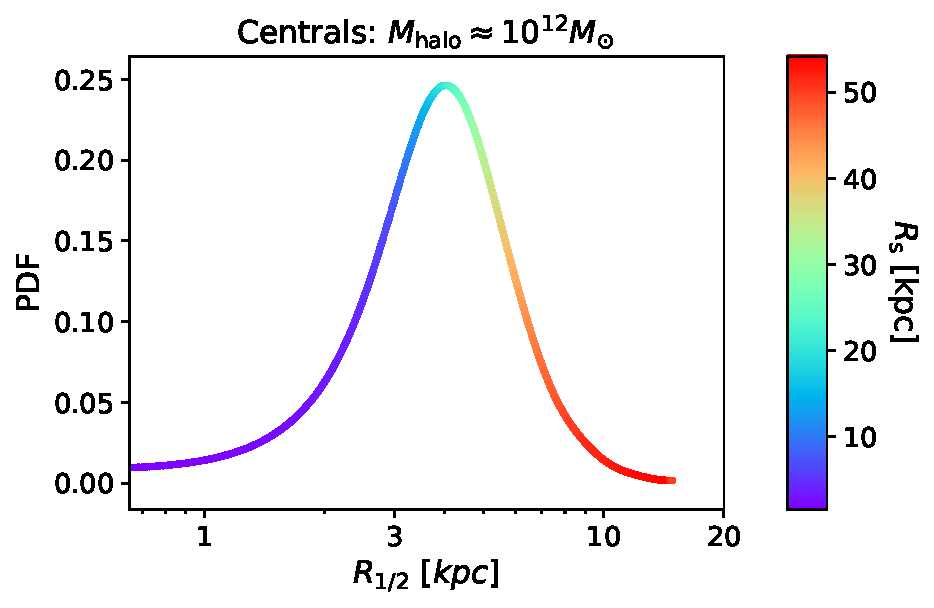
\includegraphics[width=8cm]{FIGS/rs_correlation_visual.pdf}
\caption{
{\bf Profile co-evolution model.} In this model, the log-normal distribution of galaxy sizes is determined by $\rmpeak,$ the physical size of the halo virial radius at the time the halo reaches its peak mass. Thus log-normal the shape of this curve is determined by $\langle\rhalf\vert\rmpeak\rangle=0.0125\rmpeak$ with $0.2$ dex of scatter. The profile co-evolution model further supposes that galaxy and halo profiles co-evolve across cosmic time. Thus within this log-normal distribution, for two halos with the same $\rmpeak,$ halos with larger scale radius at $\zpeak$ will host galaxies with above-average $\rhalf,$ and conversely for halos with smaller values of $\rspeak.$
}
\label{fig:coevolutionmodel}
\end{figure}
%-----------------------------------------------------------------------------------------------------

\subsubsection{$\mstar-$stripping model}
\label{subsubsec:strippingmodel}

As we will show in \S\ref{sec:results}, the chief ingredient needed to recover the observed clustering properties of galaxies is that satellites need to be smaller than centrals of comparable halo mass. Thus it is natural to consider a class of models in which stellar mass is stripped from satellite galaxies after infall.

The basis of this class of models is the fitting function presented in \citet{smith_etal16}, which was calibrated by studying stellar mass loss in a suite of high-resolution hydrodynamical simulations. In this model, $f_{\ast}$ quantifies the fraction of stellar mass lost as a function of $f_{\rm DM},$ the amount of dark matter that has been stripped since infall:

\beq
f_{\ast} = 1 - \exp(-14.2f_{\rm DM})
\eeq
For $f_{\rm DM}$ we use the ratio of present-day subhalo mass divided by the peak mass, $M_{\rm vir}/M_{\rm peak}.$ If we denote the post-stripping stellar mass as $M_{\ast}',$ then we have $M_{\ast}'\equiv f_{\ast}M_{\ast},$ where $M_{\ast}$ is given by Eq.~\ref{eq:smhm}. We then calculate the post-stripping radius by interpolating $\langle\rhalf'\vert\mstar'\rangle$ directly from SDSS data.

\section{Results}
\label{sec:results}

In Figure \ref{fig:scatter_plot} we show the scaling of galaxy size $\rhalf$ with $\mstar.$ The black curve enveloped by the gray bands show the scaling relation for our SDSS galaxy sample, while the blue curve shows the median relation $\langle\rhalf\vert\mstar\rangle$ implied by the profile co-evolution model described in \S\ref{sec:model}. This figure shows that models in which $\rhalf\propto\rvir$ can naturally give rise to the characteristic curvature in the $\langle\rhalf\vert\mstar\rangle$ relation, confirming the results in \citet{kravtsov13} in a forward modeling context.

%---------------------------------------------------------------------------------------------------
\begin{figure}
\centering
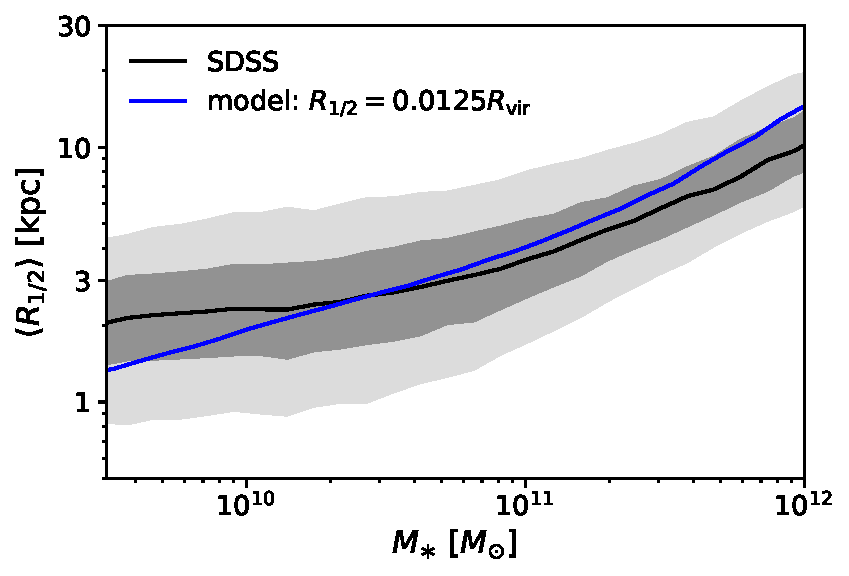
\includegraphics[width=8cm]{FIGS/rhalf_vs_mstar_fiducial_model.pdf}
\caption{The black curve shows the median $\rhalf-\mstar$ relation SDSS galaxies as measured in \citet{meert_etal15}. The two gray bands enveloping the black curve show the $50\%$ and $90\%$ percentile regions. The blue curve shows profile co-evolution model in which $\langle\rhalf\vert\rvir\rangle=0.0125\rvir,$ as in \citet{kravtsov13}. This figure confirms that a linear relationship between $\rvir$ and $\rhalf,$ convolved against the nonlinear relationships between $\rvir, \mhalo$ and $\mstar,$  predicts the characteristic curvature in the relation $\langle\rhalf\vert\mstar\rangle$ over a wide range in mass.
}
\label{fig:scatter_plot}
\end{figure}
%-----------------------------------------------------------------------------------------------------

\subsection{Size-Dependent Clustering}
\label{subsec:clustering_results}

In Figure \ref{fig:clustering_ratio_upshot} we present new measurements of the $\rhalf-$dependence of projected galaxy clustering, $\wproj(\rproj).$ Because galaxy clustering has well-known dependence upon $\mstar$ that is not the subject of this work, we wish to remove this influence and focus purely on the relationship between $\rhalf$ and $\wproj(\rproj).$ To do so, we determine the value $\langle\rhalf\vert\mstar\rangle$ by computing a sliding median of $\rhalf,$ calculated using a window of width $N_{\rm gal}=1000.$ Each galaxy is categorized as either ``large" or ``small" according to whether it is above or below the median value appropriate for its stellar mass. Using this technique, we stress that for any $\mstar-$threshold sample, the SMF of the ``large" and ``small" subsamples are identical, by construction.

We measure $\wproj(\rproj)$ separately for large and small subsamples for four different $\mstar$ thresholds, $\mstar>10^{9.75}\msun,$ $\mstar>10^{10.25}\msun,$ $\mstar>10^{10.75}\msun,$ and $\mstar>10^{11.25}\msun.$ We make the same measurements for each volume-limited $\mstar-$threshold sample {\em without} splitting on size, giving us measurements $\wpall, \wplarge,$ and $\wpsmall$ for each threshold sample. This allow us to compute the ratio $(\wplarge-\wpsmall)/\wpall,$ which we refer to as {\em the $\rhalf$ clustering ratio}. These ratios are the measurements appearing on the y-axis in each panel of Figure \ref{fig:clustering_ratio_upshot}. Points with jackknife-estimated error bars show SDSS measurements, solid curves show the clustering ratios of model galaxies as predicted by the models described in \S\ref{sec:model}.

%---------------------------------------------------------------------------------------------------
\begin{figure}
\centering
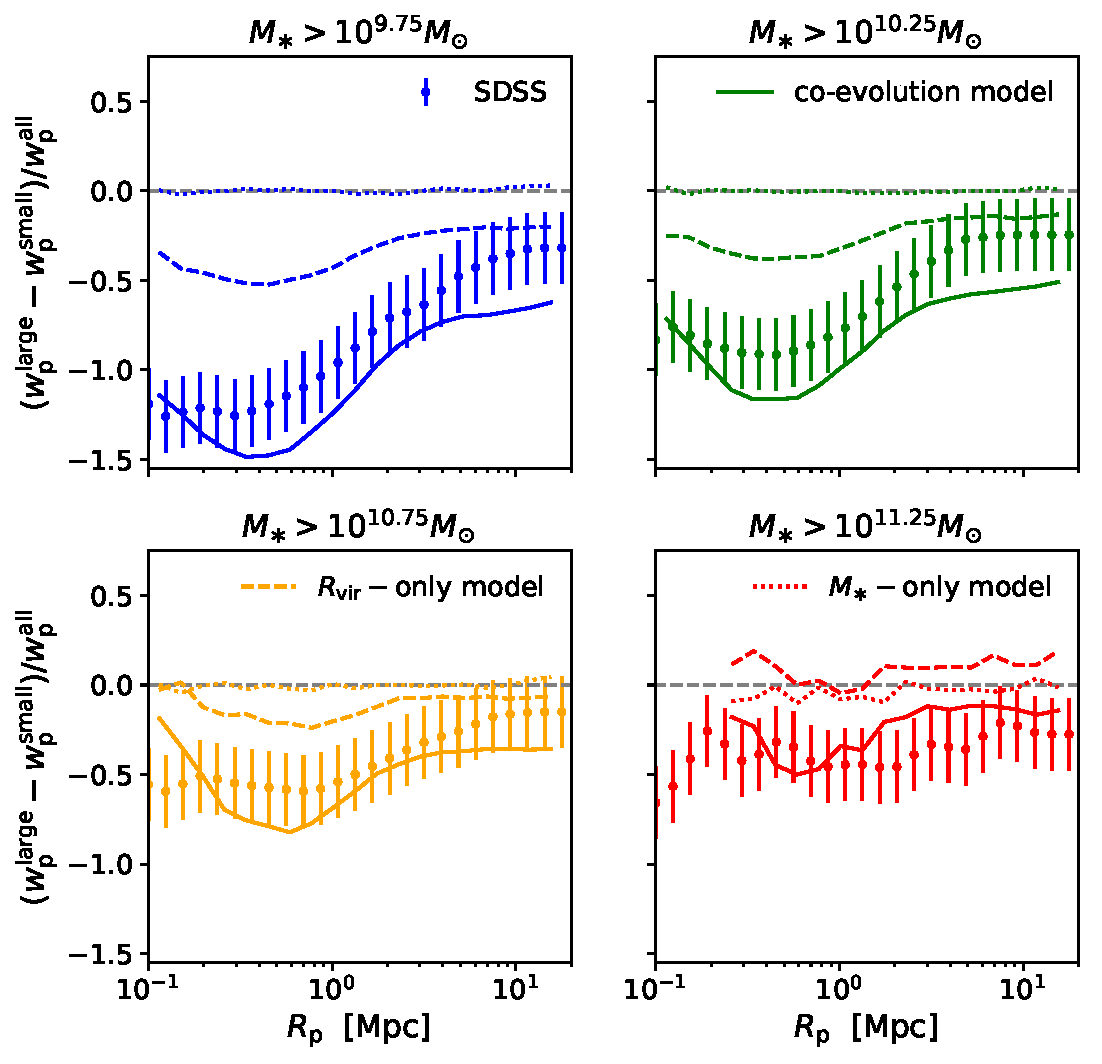
\includegraphics[width=8cm]{FIGS/penultimate_clustering_ratios_no_orphans.pdf}
\caption{
{\bf $\rhalf-$dependence of galaxy clustering.}
Points with error bars show new SDSS measurements of the $\rhalf-$dependence of projected galaxy clustering, $\wproj.$ We define a galaxy as ``large" or ``small" according to whether it is above or below the median size for its stellar mass, so that in each panel, the stellar mass functions of the ``large" and ``small" subsamples are identical, as described in the text. The y-axis shows {\em clustering strength ratios,} so that, for example, a y-axis value of $-0.5$ corresponds to small galaxies being $50\%$ more strongly clustered than large galaxies of comparable stellar mass. Each panel shows results separately for different volume-limited $\mstar-$threshold samples; predictions of three different models are shown in each panel. See \S\ref{subsec:model} for a description of each model.}
\label{fig:clustering_ratio_upshot}
\end{figure}
%-----------------------------------------------------------------------------------------------------

The salient feature of the clustering ratio measurements is that they are negative: small galaxies cluster more strongly than large galaxies of the same stellar mass, a new result. This feature also holds true for galaxies predicted by the $\rvir-$only model. This result may be surprising, since $\rhalf\propto\rvir,$ halo mass $\rvir\propto\mhalo^{1/3},$ and clustering strength increases with $\mvir.$ Based on this simple argument, one would expect the opposite trend to the measurements shown here.

\subsection{Central vs. Satellite Sizes}
\label{subsec:censat_sizes}

A straightforward resolution to the above puzzle is shown in Figure \ref{fig:censatsizehist}, which compares the $\rhalf$ distributions of central, satellite, and splashback galaxies with the same halo mass $\mpeak\approx10^{12}\msun.$ A ``splashback" galaxy is defined as a present-day central that used to be a satellite, i.e., its main progenitor halo passed inside the virial radius of a larger halo at some point in its past history. On the other hand, we define a ``true central" as a galaxy that has never been a satellite.

In the $\rvir-$only model, satellite and splashback galaxies are smaller than centrals of the same halo mass due to the physical size of their halo being smaller at earlier times $\zpeak.$ There are two distinct reasons why this feature results in small galaxies being more strongly clustered relative to larger galaxies of the same mass. First, satellite galaxies statistically occupy higher mass host halos that are more strongly clustered. In models where satellites are smaller than centrals, for any given $\mstar-$threshold the ``small" subsample will naturally have a higher satellite fraction, resulting in a negative clustering ratio as seen in SDSS data. Second, at fixed mass, halos of $L_\ast$ galaxies that form earlier are more strongly clustered, a phenomenon commonly known as {\em halo assembly bias}. Since splashback halos are typically earlier forming than true centrals, then models where splashback halos host smaller-than-average galaxies will naturally predict negative clustering ratios.

In the $\mstar-$only model, in which $\rhalf$ is statistically set by present-day stellar mass with no other dependencies. Thus neither of the above features are present: satellites and centrals of the same mass have no differences in size, and there is essentially no $\rhalf-$dependence to galaxy clustering, in gross disagreement with our SDSS observations.

Much more successful is the profile co-evolution model shown with the solid curves in Figure \ref{fig:clustering_ratio_upshot}. The strongly negative clustering ratios predicted by the assumption of profile co-evolution can be understood in terms of the same features discussed above. Figure \ref{fig:coevolutionmodel} shows that at fixed $\mpeak,$ larger galaxies will occupy halos with larger $\rspeak.$ Since halo concentration $c=\rvir/R_{\rm s},$ this implies that high-concentration galaxies will tend to host smaller galaxies. Both satellites and splashback centrals have higher concentration than true centrals, another manifestation of assembly bias, and so the assumption of profile co-evolution naturally results in an enhancement of the clustering ratios beyond the $\rvir-$only model.

\subsection{Tidal Stripping and Orphan Satellites}
\label{subsec:orphan_stripping}

We conclude this section with a discussion of Figure \ref{fig:strippingorphans}, which provides an estimate of how satellite mass stripping and orphan galaxies impact size-dependent clustering ratios. In the $\mstar-$stripping model described in \S\ref{subsubsec:strippingmodel}, satellites lose stellar mass in a way that mimics what is seen in high-resolution hydrodynamical simulations. This naturally results in an enhancement of size differences between satellites and centrals, and the dot-dashed curves in Figure \ref{fig:strippingorphans} show that produces the expected sign of the effect on the clustering ratios. The magnitude of the effect, however is not strong enough to remedy the discrepancy of the clustering predictions of the $\rvir-$only model. We discuss the physical implications of this result in \S\ref{subsec:satellite_discussion}.

The dotted curves in Figure \ref{fig:strippingorphans} show results of the $\rvir-$only model applied to a subhalo catalog that includes a orphan halos. As described in \S\ref{}, orphan halos are subhalos that are no longer resolved by {\tt Rockstar}, but whose evolution is tracked in a post-processing phase. We apply the same mass-stripping model described in \S\ref{subsubsec:strippingmodel} to this subhalo catalog that includes orphan halos, keep all model galaxies that retain more than half of their stellar mass, and show results for the $\rvir-$only model applied to the resulting catalog.

As the orphan catalog has a higher satellite fraction than the standard subhalo catalog, the negative boost shown the dotted curves in Figure \ref{fig:strippingorphans} is expected. Orphan halos also typically have earlier-than-average values of $\zpeak$ relative to ordinary subhalos, which also enhances differences between central and satellite sizes. See \S\ref{subsec:satellite_discussion} for further discussion.

%---------------------------------------------------------------------------------------------------
\begin{figure}
\centering
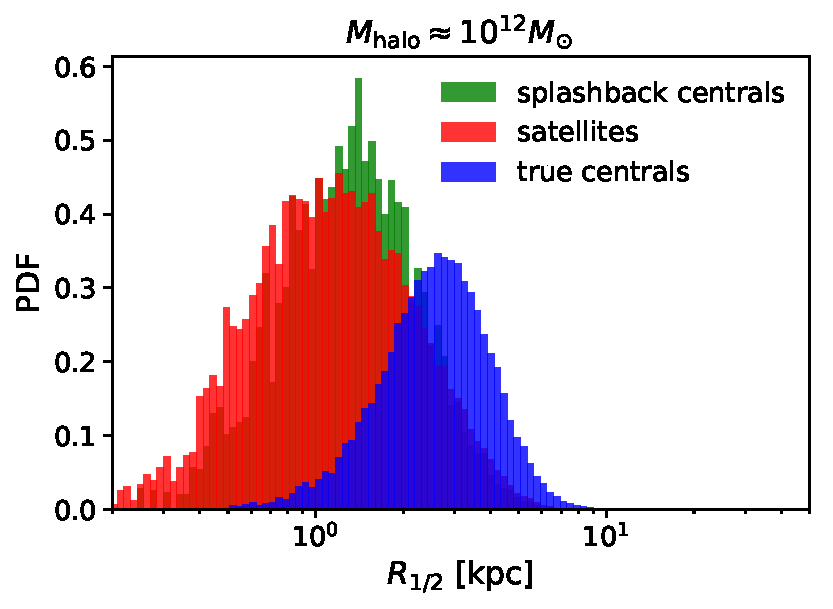
\includegraphics[width=8cm]{FIGS/cen_sat_sizes.pdf}
\caption{
{\bf Relative sizes of centrals and satellites.} In a narrow bin of halo mass $\mhalo=\mpeak\approx10^{12}\msun,$ we show the distribution of model galaxy sizes for different subpopulations galaxies, as predicted by the $\rvir-$only model. The red histogram shows the sizes of satellites; the blue histogram shows host halos that have never passed inside the virial radius of a larger halo (``true centrals"); the green histogram host halos that were subhalos inside a larger at some point in their past history (``splashback halos"). In the $\rvir-$only model, galaxy size is set by the {\em physical} size of the virial radius at the time the halo attains its peak mass, naturally resulting in smaller sizes for satellites and backsplash centrals relative to true centrals of the same $\mpeak.$ The central/satellite size differences shown here are not enough to correctly predict the observed clustering ratios (see Figure \ref{fig:clustering_ratio_upshot}), motivating the $\mstar-$stripping and profile co-evolution models.
}
\label{fig:censatsizehist}
\end{figure}
%-----------------------------------------------------------------------------------------------------

%---------------------------------------------------------------------------------------------------
\begin{figure}
\centering
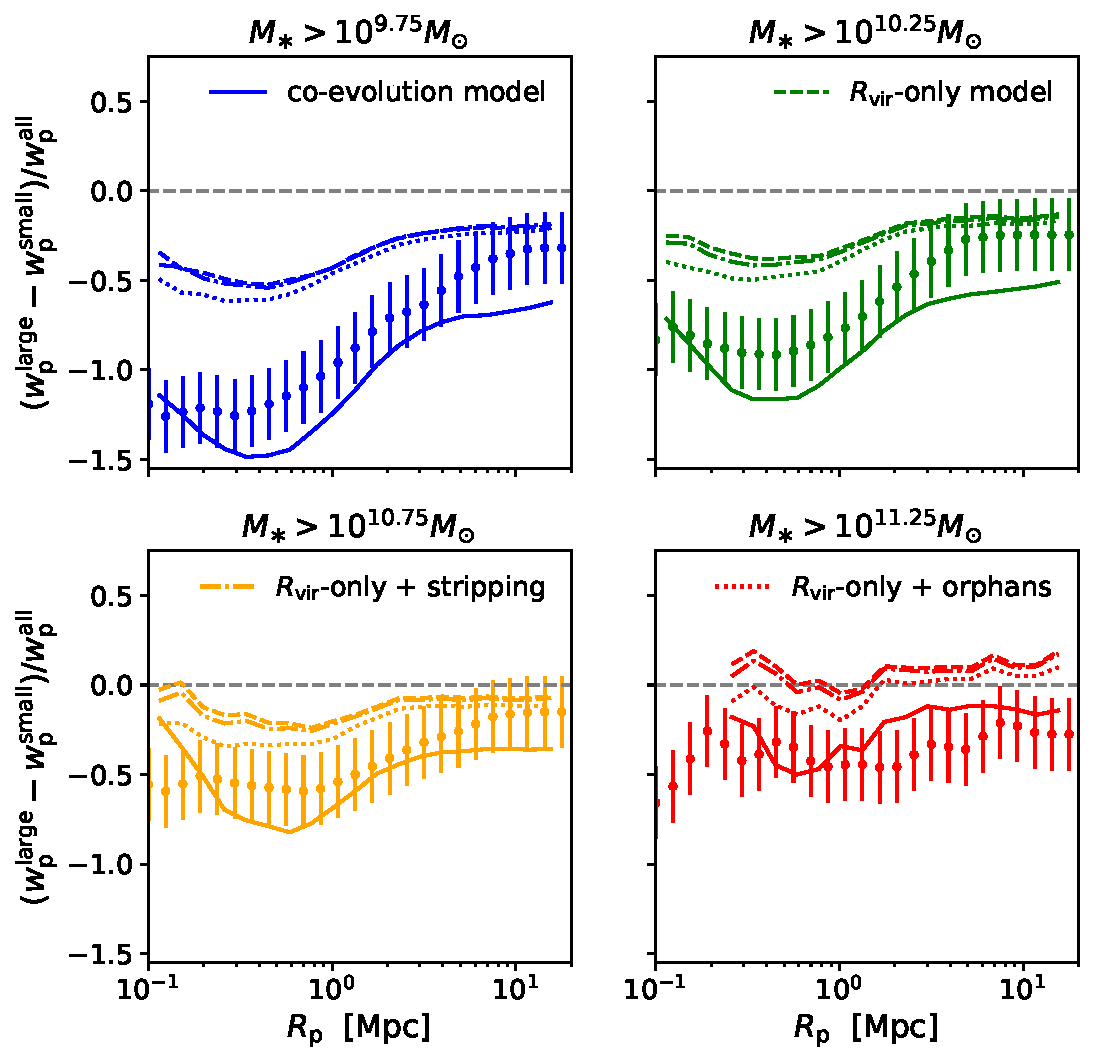
\includegraphics[width=8cm]{FIGS/penultimate_clustering_ratios_alternate_models.pdf}
\caption{
{\bf Impact of tidal stripping and orphan satellites.} In all panels, the axes and points with error bars are the same as in Figure \ref{fig:clustering_ratio_upshot}. The dashed curves (``$\rvir-$only model") and solid curves (``profile co-evolution model") from  Figure \ref{fig:clustering_ratio_upshot} are also shown for convenience. The dot-dashed curves show results for a model in which satellites lose mass after infall in a manner similar to what is seen in high-resolution hydrodynamical simulations, as described in \S\ref{subsubsec:strippingmodel}. The dotted curve shows results for the same model, but including the effect of ``orphan" galaxies that live in subhalos no longer resolved by {\tt Rockstar}.
}
\label{fig:strippingorphans}
\end{figure}
%-----------------------------------------------------------------------------------------------------

\section{Discussion}
\label{sec:discussion}

\subsection{Progression from Backwards to Forward Modeling}
\label{subsec:forwardsmodeling}

Our results give an archetypal demonstration of the natural scientific progression from backwards to forward modeling. In backwards modeling, some mapping is applied to observed galaxies to estimate the values of model quantities such as halo mass. In \citet{kravtsov13}, the model quantities mapped onto galaxies are $\mhalo$ and $\rvir;$ another classic example of backwards modeling uses a group- or cluster-finding algorithm to assign $\mhalo$ to observed galaxies \citep[e.g.,][]{berlind_etal06,yang_etal05a,rykoff_etal14}. Once the observed galaxies have been supplemented with model variables, then the relations of the galaxy-halo connection can be inferred, for example, by calculating quantities such as the mean stellar mass or quiescent fraction as a function of halo mass \citep[e.g.,][]{yang_etal05b,weinmann_etal06}.

In forward modeling, the direction of inference is turned around: a mapping is instead applied to the model quantities such as $\mhalo.$ In the case of {\tt Halotools}, this transforms a cosmological simulation into a synthetic galaxy catalog that can be directly compared with observations. This enables a richer quantitative study of modeling hypotheses relative to backwards modeling. For example, Figure \ref{fig:clustering_ratio_upshot} shows how forward modeling allows us to exploit galaxy clustering measurements to quantitatively test whether $\mhalo$ or $\mstar$ is the statistical regulator of galaxy size. The ability disentangle coupled variables such as $\mstar$ and $\mhalo$ is just one example of this advantage of forward modeling. Another example is illustrated in Figure \ref{fig:censatsizehist}, in which we explore the role of splashback halos in setting galaxy size. In our forward modeling approach, this is entirely straightforward; in backwards modeling, such an investigation would not even be possible without introducing additional modeling ingredients.

Backwards modeling the galaxy-halo connection is useful for generating hypotheses and motivating functional forms. Forward modeling becomes necessary when the problem at hand becomes encumbered by multiple relevant variables, as is the case with galaxy size. Forward modeling also makes it possible to conduct rigorous Bayesian inference, which we consider to be the next natural step in the progression described here (see \S\ref{subsec:future} for further discussion).

\subsection{Relation to Previous Work}
\label{subsec:previous_work}

Backwards modeling methods have been used extensively in the literature to gain insight into the relationship between galaxy mass, size, and environment. Broadly speaking, such studies proceed by using a galaxy group catalog to classify observed galaxies as centrals or satellites, and estimate their halo mass.  Employing such methods, several analyses of the \citet{yang_etal05b} group catalog have found that the $\mstar-\rhalf$ relation of early-type galaxies exhibits weak, if any, environmental dependence \citep{huertas_company_etal13b,shankar_etal14}. 

A direct comparison to this finding is not possible because the conclusions drawn here pertain to $\mstar-$limited galaxy samples. As discussed in \citet{spindler_wake17}, it is entirely possible that size differences between centrals and satellites of the same mass can be accounted for by mutual covariance with an additional variable such as star formation rate or morphological type \citep[see also][for an explicit demonstration of this scenario]{lilly_carollo16}. In particular, suppose that centrals and satellites of the same mass have different early-type fractions as indicated in \citet{weinmann_etal06}, and that early- and late-type galaxies exhibit universal, but distinct, $\mstar-\rhalf$ relations. In such a case, centrals would be larger than satellites of the same mass, even though {\em early-type centrals} would have the same sizes as {\em early-type satellites}. 

As discussed in \S\ref{subsec:future}, we are currently pursuing follow-up work in which we jointly model morphological type together with galaxy size. We consider forward modeling methods to be a requisite for progress on this issue, not only to properly handle the multi-dimensional nature of the problem, but also to rigorously treat systematic errors that plague inference based on galaxy group catalogs \citep[see][for a thorough discussion]{campbell_etal15}. 

Our approach is closely aligned with the methods used in \citet{somerville_etal17}, who studied the empirical modeling features that are necessary to recover the tight scatter in the observed $\langle\rhalf\vert\mstar\rangle$ relation. By building models where $\rhalf$ is set by halo spin $\lambda_{\rm halo}$, the authors in \citet{somerville_etal17} found that the level of intrinsic scatter about $\langle\lambda_{\rm halo}\vert\mhalo\rangle$ in dark matter halos is at least as large as the scatter about $\langle\rhalf\vert\mstar\rangle$ seen in observed galaxies. Since the latter necessarily receives an additional contribution from measurement error, this implies some tension with the common semi-analytic modeling assumption that $\lambda_{\rm halo}$ scales with $\rhalf.$ As noted in \citet{somerville_etal17}, tension in the level of scatter cannot be used to directly test the $\lambda_{\rm halo}\propto\rhalf$ assumption because the physical motivation for this correlation is largely limited to disk galaxies \citep{mo_mao_white98}. This tension is not present in our approach for the reason that the level of scatter is simply a modeling parameter in our approach, and we make no attempt to uncover the physical origin of this scatter. However, our fiducial value choice was motivated by \citet{somerville_etal17}, and in the ongoing follow-up work discussed in \S\ref{subsec:future} we will systematically test the large-scale structure implications of the assumption that $\lambda_{\rm halo}\propto\rhalf^{\rm disk}.$

\subsection{Implications for Satellite Evolution}
\label{subsec:satellite_discussion}

Explanations for differences between the sizes of centrals and satellites fall into two categories, depending on whether or not the processes involved are specific to post-infall physics. One obvious possibility that could lead to satellites being smaller than centrals of the same $\mhalo$ is tidal stripping: satellite $\mstar$ could decrease after infall, reducing the size of the galaxy. We have quantitatively tested this possibility with the $\mstar-$stripping model described in \S\ref{subsubsec:strippingmodel}. Comparing the clustering ratios of the ``$\rvir-$only" and ``$\rvir+$stripping" models in Figure \ref{fig:strippingorphans}, we find that the impact of physically motivated levels of satellite mass loss cannot explain the $\rhalf-$dependent clustering seen in SDSS. As an additional test, we reach the same conclusion when implementing an even more extreme $\mstar-$stripping model in which stellar mass loss is linearly proportional to halo mass loss \citep[][Model 1]{watson_etal12}. 

Both the $\rvir-$only model and the co-evolution model (see sections \S\ref{subsubsec:rvirmodel} and \S\ref{subsubsec:coevolutionmodel}, respectively) represent explanations falling into the second category, in which centrals and satellites of the same $\mhalo$ have different sizes due to their different evolutionary paths {\em prior} to satellite infall. For these models the story is very different: the influence of pre-infall co-evolution has a dramatic impact on $\rhalf-$clustering ratios, with a scale- and $\mstar-$dependence that closely resembles the SDSS signal. Quantitative constraints on the true level of this co-evolution effect will be a natural outcome of the program described in \S\ref{subsec:future}, but it is already clear that the long term co-evolution of galaxy and halo profiles should be considered a critical ingredient to models for the distribution of galaxy sizes across the cosmic web. 

\subsection{Future Directions for Empirical Modeling of Galaxy Size}
\label{subsec:future}

\subsubsection{Jointly modeling $\langle\mstar\vert\mhalo\rangle$}

The scope of this work is to serve as a pilot study in which we identify the chief ingredients that can influence the $\rhalf-$dependence of galaxy clustering. While our results suggest that our profile co-evolution model is giving the correct qualitative picture, our implementation cannot be correct in quantitative detail: the clustering ratios of this model shown in Figure \ref{fig:clustering_ratio_upshot} are too strong relative to SDSS. This likely indicates that the central/satellite size differences depicted in Figure \ref{fig:} are too strong, and that the correlation strength in the real Universe is intermediate, rather than maximal. Our publicly available code that reproduces our results already contains the machinery to implement continuously variable levels of $\rhalf-\rspeak$ correlation strength, but for present purposes we have chosen to focus on exploring bracketing cases of qualitative ingredients, rather than fine-tuning the model. 

In addition to varying the $\rhalf-\rspeak$ correlation strength, there are other factors that should be included in any proper likelihood analysis of galaxy size models. In particular, since the clustering signal is strongly influenced by differences between centrals and satellites, then the satellite fraction $F_{\rm sat}(\mstar)$ plays an important role in $\rhalf-$dependent clustering. For fixed scaling relations $\langle\rhalf^{\rm cens}\vert\mhalo\rangle$ and $\langle\rhalf^{\rm sats}\vert\mhalo\rangle,$ models with different satellite fractions will exhibit different $\rhalf-$clustering ratios because $F_{\rm sat}(\mstar)$ controls the relative weighting of the two populations. Our results based on the catalog that includes orphan subhalos (Figure \ref{fig:strippingorphans}, dotted curves) give an explicit demonstration of the impact of $F_{\rm sat}(\mstar)$ on the clustering signal. 

On the one hand, this degeneracy with the satellite fraction is unfortunate, because it means galaxy sizes does not leave a pure and unique signature on $\rhalf-$clustering ratios. However, this can also be viewed as an opportunity to extract tighter constraints on $F_{\rm sat}(\mstar),$ which are sorely needed to discriminate between competing models. For this problem, the path forward is clear. Traditional galaxy clustering is already being used to validate and/or fit models of the stellar-to-halo-mass relation \citep[e.g.,][]{moster_etal13,behroozi13_smhm,lehmann_etal15}. Based on our results, we advocate that empirical models for $\langle\mstar\vert\mhalo\rangle$ be supplemented with additional model ingredients for $\langle\rhalf\vert\mstar\rangle,$ and that the parameters of composite model are jointly constrained by measurements of the stellar mass function, $\mstar-$dependent clustering, and $\rhalf-$dependent clustering. Careful attention will need to be paid to the orphan subhalo population, which is well-known to have a significant impact on small-scale clustering \citep{guo_white13,campbell_etal17}. 

\subsubsection{Jointly modeling morphology}

Previous studies of large-scale structure measured by SDSS indicate that morphological type has a significant influence on galaxy clustering \citep{skibba_etal08}. Because morphology is covariant with star-formation rate (SFR) and $\rhalf,$ accounting for this dependency will require simultaneously modeling each of these variables. 

To date, such a task has been beyond the purview of empirical models. However, recent progress has substantially improved the richness of the predictions that galaxy-halo models are capable of \citep{becker15,cohn17,moster_etal17}. This new class of models has accomplished this by empirically modeling star-formation rate, and then integrating SFR along each halo's history to differentially build up stellar mass.\footnote{This approach towards predicting $\mstar$ is thus mathematically akin to traditional semi-analytic models, although \citet{becker15} have retained the empirical modeling prioritization of simplicity and computational efficiency.} We are currently extending this new class of models to differentially build up the disk and bulge across cosmic time. In addition to treating the multi-dimensional nature of the problem, this also allows us to use data at higher redshift in a self-consistent manner.  


\section{Conclusions}
\label{sec:conclusion}

We have presented new measurements of the dependence of galaxy clustering upon galaxy size, and used {\tt Halotools} to identify the basic ingredients that influence the signal. We conclude with a brief summary of our primary findings:

\ben
\item Small galaxies cluster more strongly than large galaxies of the same stellar mass, a new result. Differences between the clustering of small and large galaxies increase on small scales $R\lesssim1\mpc,$ and decrease with stellar mass.
\item The most important ingredient influencing this signal is the relative size of central and satellite galaxies. The magnitude, scale-dependence, and $\mstar-$dependence of $\rhalf-$dependent clustering provides strong evidence that satellite galaxies are smaller than central galaxies of the same halo mass.
\item Simple empirical models in which $\rhalf$ is regulated by $\mstar,$ rather than $\mhalo,$ are grossly discrepant with the observed clustering signal.
\item The ``co-evolution model" shown with solid curves in Figure \ref{fig:clustering_ratio_upshot} exhibits a clustering signal that is strikingly similar to that seen in SDSS. In this model, $\rhalf$ is statistically regulated by $\rmpeak,$ the halo virial radius $\rvir$ at the time of peak halo mass, with strong residual correlation with $\rspeak,$ the halo scale radius at that time. The success of this model supports the notion that galaxy and halo profiles co-evolve across many Gyr of cosmic time.
\een

Our results can be treated as a boundary condition for more complex and fine-grained models of galaxy size, such as semi-analytic models and hydrodynamical simulations. We view the present work as a pilot study that motivates a Bayesian inference program to tightly constrain the galaxy size-halo connection with forward modeling techniques, in direct analogy to the literature on the stellar-to-halo-mass relation. Our publicly available code provides a simple means for cosmological surveys to generate synthetic galaxy populations with realistic sizes across the cosmic web.

\section*{Acknowledgments}

APH thanks John Baker for the {\em Toejam \& Earl} soundtrack. Thanks also to Frank van den Bosch, Doug Watson, and Risa Wechsler for thoughtful feedback at various stages of the development of this work.

We thank the {\tt Astropy} developers for the package-template \citep{astropy}, and {\tt NumPy} \citep{numpy_ndarray}, {\tt SciPy} \citep{scipy}, IPython, Matplotlib, and GitHub for their extremely useful free software.

This research was supported in part by the National Science Foundation under Grant No. NSF PHY11-25915. Work done at Argonne National Laboratory was supported under the DOE contract DE-AC02-06CH11357.

\bibliography{galsize_paper}

\end{document}







